\chapter{Evaluation and Results}
This chapter describes the experimental process of this camera calibration method and the equipment used for the experiments. Furthermore, all the system parameters and results are also demonstrated in detail. Even though the system contains 16 cameras, we worked with four cameras in this experiment scope to test the calibration method. If the experiment result is accurate, we will gradually increase the number of cameras for further experiments.

\clearpage
\section{Overview}
Firstly, this chapter mentions the equipment necessary for the experiment, especially the cameras and the double-sided ArUco board. Cameras with their intrinsic parameters, as well as the ArUco board configuration, are defined clearly. 

This chapter then demonstrates the extrinsic calibration process for each camera. In order to optimise the calibration result, each camera continuously captures the image of the ArUco board and estimates the board's transformation respecting to the camera frame during the calibration process.
Finally, the set of estimated board poses of the whole camera system from the previous stage is processed by the General Graph Optimisation (G2O) framework. This framework aggregates the detected board's poses of the entire procedure and then calculates the final extrinsic parameters between cameras in the system.

This experiment's program framework and algorithm are mainly programmed in C++ with Open-CV 4.2.0 library. MATLAB programming language is also used to test the algorithm and initialise the ArUco board configuration. Besides, we use ROS Noetic as a middle-ware to help communicate between the camera system and our framework.

\clearpage
\section{Camera system}
For the scope and purpose of this experiment, we decide to use four RGB-D cameras Intel Realsense RGB-D D435i. This type of camera can capture images up to 1920x1080 resolution with a frame rate up to 60 Hz. The RGB-D camera can also capture depth images, which is very important for our project purpose, such as 3D reconstruction. Furthermore, the manufacturers have calibrated the intrinsic parameters of these cameras, so we just have to focus on the extrinsic calibration problem. Additionally, these cameras can be synchronised together via cable, which is important in working with multiple cameras. Intel has developed a ROS "wrapper" for the camera firmware that makes it more straightforward to communicate between the cameras and our framework, simplifying the programming for the calibration algorithm.

\begin{figure}[ht]
\centering
\includegraphics[width=0.9\textwidth]{Images/Realsense.jpg}
\caption{RGB-D Camera Intel Realsense D435i}
\end{figure}

The intrinsic parameter (also known as the camera matrix) is defined by
\[    % <-- start math environment
K =
\begin{bmatrix}
    f_{x} &  0      & c_{x} \\
    0     &  f_{y}  & c_{y} \\
    0     &  0      & 1
\end{bmatrix}
,
\]    % <-- end of math environment

in which $f_{x}$, $f_{y}$ is the focal length and $(c_{x}$, $c_{y})$ is the principal point, which is unique to each camera. After checking the manufacturer firmware, the intrinsic parameters of the four cameras in our system are listed below. We intend to store the intrinsic parameters of these cameras in a YAML file to simplify our program framework as well as be convenient for modifying the parameters without recompiling the code.

\begin{table}[ht]
    \caption{\label{tab:intrinsic}Intrinsic parameters of each camera.}
    \begin{tabular}{ |c|c|c|c|c| }
     \hline
    Cam & $f_{x}$ & $f_{y}$ & $c_{x}$ & $c_{y}$ \\
     \hline
    1 & 633.470275878906 & 633.470275878906 & 643.229064941406 & 358.437103271484 \\ 
    2 & 637.565185546875 & 637.565185546875 & 643.337707519531 & 355.360290527343 \\
    3 & 640.793884277343 & 640.793884277343 & 645.108825683593 & 356.419738769531 \\ 
    4 & 642.689758300781 & 642.689758300781 & 645.234985351562 & 355.756347656250 \\ 
     \hline
    \end{tabular}
\end{table}

\begin{figure}[ht]
\centering
\includegraphics[width=1\textwidth]{Images/Camera layout.png}
\caption{Camera layout}
\end{figure}

\clearpage
\section{Double-sided ArUco board configuration}
In this experiment, firstly, we use a wood panel with an exact thickness of 6.6 millimetres (measured carefully). The board should be large enough to fit an A3 paper containing a set of ArUco markers, as well as make it easier for cameras to detect the board's features.

Secondly, we decided to use 56 ArUco markers with IDs from 0 to 55, which means 28 tags on each side of the board. The markers' size is 4x4, composed of 16 binary bits. All 56 markers are printed on two sheets of A3 size paper, with 28 markers each, ordered from left to right and top to bottom with four rows and seven columns. Each marker is a square with a four-centimetre side length, and the gap between each marker is two centimetres. We use Microsoft Publisher to design the ArUco board before printing to ensure the size of each marker, as well as the distance between the markers, is correct. Additionally, when sticking on the wood board, we must guarantee that the markers on the two sides match together precisely.

 \begin{figure}[ht]
 \centering
 \includegraphics[width=1\textwidth]{Images/Double-sided ArUco board (front side).jpg}
 \caption{Double-sided ArUco board (front side)}

 \vspace{10mm}

 \includegraphics[width=1\textwidth]{Images/Double-sided ArUco board (back side).jpg}
 \caption{Double-sided ArUco board (back side)}
 \end{figure}

\clearpage
Finally, we have to initialise the parameters of the ArUco board configuration. As mentioned above, a board's layout includes three essential parameters: IDs of markers, the object points and the dictionary. IDs are numbered from 0 to 55, and each ID represents a marker on the board. Because the ArUco markers we are using have a 4x4 size and the total of tags used is 56, we decided to use the dictionary DICT\_4X4\_100 (each dictionary is contained a different amount of ArUco tags). About the object points, we use a MATLAB script to generate a list of object points belonging to the markers (the table below). Thanks to Mr Jasprabhjit Mehami for the support on this Matlab script.

The origin coordinate of the whole board is located at the bottom-left corner of ArUco marker ID number 21. Board's thickness is 6.6 millimetres (0.0066 meters), so all the ArUco markers located on the backside have the z-coordinate of corners equal to -0.0066 (which is respected to the board origin coordinate).

\clearpage
\begin{footnotesize}
\begin{longtable}{|l|l|l|l|l|l|l|l|l|l|l|l|l|}
\caption{\normalsize \label{tab:boardconfig}Double-sided ArUco board configuration} \\
\hline
IDs & x    & y    & z       & x    & y    & z       & x    & y    & z       & x    & y    & z       \\ \hline
\endfirsthead
\endhead
%
0   & 0    & 0.22 & 0       & 0.04 & 0.22 & 0       & 0.04 & 0.18 & 0       & 0    & 0.18 & 0       \\ \hline
1   & 0.06 & 0.22 & 0       & 0.1  & 0.22 & 0       & 0.1  & 0.18 & 0       & 0.06 & 0.18 & 0       \\ \hline
2   & 0.12 & 0.22 & 0       & 0.16 & 0.22 & 0       & 0.16 & 0.18 & 0       & 0.12 & 0.18 & 0       \\ \hline
3   & 0.18 & 0.22 & 0       & 0.22 & 0.22 & 0       & 0.22 & 0.18 & 0       & 0.18 & 0.18 & 0       \\ \hline
4   & 0.24 & 0.22 & 0       & 0.28 & 0.22 & 0       & 0.28 & 0.18 & 0       & 0.24 & 0.18 & 0       \\ \hline
5   & 0.3  & 0.22 & 0       & 0.34 & 0.22 & 0       & 0.34 & 0.18 & 0       & 0.3  & 0.18 & 0       \\ \hline
6   & 0.36 & 0.22 & 0       & 0.4  & 0.22 & 0       & 0.4  & 0.18 & 0       & 0.36 & 0.18 & 0       \\ \hline
7   & 0    & 0.16 & 0       & 0.04 & 0.16 & 0       & 0.04 & 0.12 & 0       & 0    & 0.12 & 0       \\ \hline
8   & 0.06 & 0.16 & 0       & 0.1  & 0.16 & 0       & 0.1  & 0.12 & 0       & 0.06 & 0.12 & 0       \\ \hline
9   & 0.12 & 0.16 & 0       & 0.16 & 0.16 & 0       & 0.16 & 0.12 & 0       & 0.12 & 0.12 & 0       \\ \hline
10  & 0.18 & 0.16 & 0       & 0.22 & 0.16 & 0       & 0.22 & 0.12 & 0       & 0.18 & 0.12 & 0       \\ \hline
11  & 0.24 & 0.16 & 0       & 0.28 & 0.16 & 0       & 0.28 & 0.12 & 0       & 0.24 & 0.12 & 0       \\ \hline
12  & 0.3  & 0.16 & 0       & 0.34 & 0.16 & 0       & 0.34 & 0.12 & 0       & 0.3  & 0.12 & 0       \\ \hline
13  & 0.36 & 0.16 & 0       & 0.4  & 0.16 & 0       & 0.4  & 0.12 & 0       & 0.36 & 0.12 & 0       \\ \hline
14  & 0    & 0.1  & 0       & 0.04 & 0.1  & 0       & 0.04 & 0.06 & 0       & 0    & 0.06 & 0       \\ \hline
15  & 0.06 & 0.1  & 0       & 0.1  & 0.1  & 0       & 0.1  & 0.06 & 0       & 0.06 & 0.06 & 0       \\ \hline
16  & 0.12 & 0.1  & 0       & 0.16 & 0.1  & 0       & 0.16 & 0.06 & 0       & 0.12 & 0.06 & 0       \\ \hline
17  & 0.18 & 0.1  & 0       & 0.22 & 0.1  & 0       & 0.22 & 0.06 & 0       & 0.18 & 0.06 & 0       \\ \hline
18  & 0.24 & 0.1  & 0       & 0.28 & 0.1  & 0       & 0.28 & 0.06 & 0       & 0.24 & 0.06 & 0       \\ \hline
19  & 0.3  & 0.1  & 0       & 0.34 & 0.1  & 0       & 0.34 & 0.06 & 0       & 0.3  & 0.06 & 0       \\ \hline
20  & 0.36 & 0.1  & 0       & 0.4  & 0.1  & 0       & 0.4  & 0.06 & 0       & 0.36 & 0.06 & 0       \\ \hline
21  & 0    & 0.04 & 0       & 0.04 & 0.04 & 0       & 0.04 & 0    & 0       & 0    & 0    & 0       \\ \hline
22  & 0.06 & 0.04 & 0       & 0.1  & 0.04 & 0       & 0.1  & 0    & 0       & 0.06 & 0    & 0       \\ \hline
23  & 0.12 & 0.04 & 0       & 0.16 & 0.04 & 0       & 0.16 & 0    & 0       & 0.12 & 0    & 0       \\ \hline
24  & 0.18 & 0.04 & 0       & 0.22 & 0.04 & 0       & 0.22 & 0    & 0       & 0.18 & 0    & 0       \\ \hline
25  & 0.24 & 0.04 & 0       & 0.28 & 0.04 & 0       & 0.28 & 0    & 0       & 0.24 & 0    & 0       \\ \hline
26  & 0.3  & 0.04 & 0       & 0.34 & 0.04 & 0       & 0.34 & 0    & 0       & 0.3  & 0    & 0       \\ \hline
27  & 0.36 & 0.04 & 0       & 0.4  & 0.04 & 0       & 0.4  & 0    & 0       & 0.36 & 0    & 0       \\ \hline
28  & 0.36 & 0.22 & -0.0066 & 0.4  & 0.22 & -0.0066 & 0.4  & 0.18 & -0.0066 & 0.36 & 0.18 & -0.0066 \\ \hline
29  & 0.3  & 0.22 & -0.0066 & 0.34 & 0.22 & -0.0066 & 0.34 & 0.18 & -0.0066 & 0.3  & 0.18 & -0.0066 \\ \hline
30  & 0.24 & 0.22 & -0.0066 & 0.28 & 0.22 & -0.0066 & 0.28 & 0.18 & -0.0066 & 0.24 & 0.18 & -0.0066 \\ \hline
31  & 0.18 & 0.22 & -0.0066 & 0.22 & 0.22 & -0.0066 & 0.22 & 0.18 & -0.0066 & 0.18 & 0.18 & -0.0066 \\ \hline
32  & 0.12 & 0.22 & -0.0066 & 0.16 & 0.22 & -0.0066 & 0.16 & 0.18 & -0.0066 & 0.12 & 0.18 & -0.0066 \\ \hline
33  & 0.06 & 0.22 & -0.0066 & 0.1  & 0.22 & -0.0066 & 0.1  & 0.18 & -0.0066 & 0.06 & 0.18 & -0.0066 \\ \hline
34  & 0    & 0.22 & -0.0066 & 0.04 & 0.22 & -0.0066 & 0.04 & 0.18 & -0.0066 & 0    & 0.18 & -0.0066 \\ \hline
35  & 0.36 & 0.16 & -0.0066 & 0.4  & 0.16 & -0.0066 & 0.4  & 0.12 & -0.0066 & 0.36 & 0.12 & -0.0066 \\ \hline
36  & 0.3  & 0.16 & -0.0066 & 0.34 & 0.16 & -0.0066 & 0.34 & 0.12 & -0.0066 & 0.3  & 0.12 & -0.0066 \\ \hline
37  & 0.24 & 0.16 & -0.0066 & 0.28 & 0.16 & -0.0066 & 0.28 & 0.12 & -0.0066 & 0.24 & 0.12 & -0.0066 \\ \hline
38  & 0.18 & 0.16 & -0.0066 & 0.22 & 0.16 & -0.0066 & 0.22 & 0.12 & -0.0066 & 0.18 & 0.12 & -0.0066 \\ \hline
39  & 0.12 & 0.16 & -0.0066 & 0.16 & 0.16 & -0.0066 & 0.16 & 0.12 & -0.0066 & 0.12 & 0.12 & -0.0066 \\ \hline
40  & 0.06 & 0.16 & -0.0066 & 0.1  & 0.16 & -0.0066 & 0.1  & 0.12 & -0.0066 & 0.06 & 0.12 & -0.0066 \\ \hline
41  & 0    & 0.16 & -0.0066 & 0.04 & 0.16 & -0.0066 & 0.04 & 0.12 & -0.0066 & 0    & 0.12 & -0.0066 \\ \hline
42  & 0.36 & 0.1  & -0.0066 & 0.4  & 0.1  & -0.0066 & 0.4  & 0.06 & -0.0066 & 0.36 & 0.06 & -0.0066 \\ \hline
43  & 0.3  & 0.1  & -0.0066 & 0.34 & 0.1  & -0.0066 & 0.34 & 0.06 & -0.0066 & 0.3  & 0.06 & -0.0066 \\ \hline
44  & 0.24 & 0.1  & -0.0066 & 0.28 & 0.1  & -0.0066 & 0.28 & 0.06 & -0.0066 & 0.24 & 0.06 & -0.0066 \\ \hline
45  & 0.18 & 0.1  & -0.0066 & 0.22 & 0.1  & -0.0066 & 0.22 & 0.06 & -0.0066 & 0.18 & 0.06 & -0.0066 \\ \hline
46  & 0.12 & 0.1  & -0.0066 & 0.16 & 0.1  & -0.0066 & 0.16 & 0.06 & -0.0066 & 0.12 & 0.06 & -0.0066 \\ \hline
47  & 0.06 & 0.1  & -0.0066 & 0.1  & 0.1  & -0.0066 & 0.1  & 0.06 & -0.0066 & 0.06 & 0.06 & -0.0066 \\ \hline
48  & 0    & 0.1  & -0.0066 & 0.04 & 0.1  & -0.0066 & 0.04 & 0.06 & -0.0066 & 0    & 0.06 & -0.0066 \\ \hline
49  & 0.36 & 0.04 & -0.0066 & 0.4  & 0.04 & -0.0066 & 0.4  & 0    & -0.0066 & 0.36 & 0    & -0.0066 \\ \hline
50  & 0.3  & 0.04 & -0.0066 & 0.34 & 0.04 & -0.0066 & 0.34 & 0    & -0.0066 & 0.3  & 0    & -0.0066 \\ \hline
51  & 0.24 & 0.04 & -0.0066 & 0.28 & 0.04 & -0.0066 & 0.28 & 0    & -0.0066 & 0.24 & 0    & -0.0066 \\ \hline
52  & 0.18 & 0.04 & -0.0066 & 0.22 & 0.04 & -0.0066 & 0.22 & 0    & -0.0066 & 0.18 & 0    & -0.0066 \\ \hline
53  & 0.12 & 0.04 & -0.0066 & 0.16 & 0.04 & -0.0066 & 0.16 & 0    & -0.0066 & 0.12 & 0    & -0.0066 \\ \hline
54  & 0.06 & 0.04 & -0.0066 & 0.1  & 0.04 & -0.0066 & 0.1  & 0    & -0.0066 & 0.06 & 0    & -0.0066 \\ \hline
55  & 0    & 0.04 & -0.0066 & 0.04 & 0.04 & -0.0066 & 0.04 & 0    & -0.0066 & 0    & 0    & -0.0066 \\ \hline
\end{longtable}
\end{footnotesize}

\clearpage
\section{Board pose estimation}
To estimate the relative pose of the ArUco board to each camera, we have to solve the Perspective-n-Point (PnP) pose problem. Due to the popularity of this problem in camera calibration, several methods are implemented and published as packages or libraries. Our program framework is mainly written in C++, so we intend to use the Open-CV library for Perspective-n-Point (PnP) pose computation.

\begin{figure}[ht]
\centering
\includegraphics[width=1\textwidth]{Images/solvePnP().jpg}
\caption{SolvePnP() function in Open-CV library in detail}
\end{figure}

In which, "objectPoints" are corner coordinates of ArUco markers respected to the board's origin, and the "imagePoints" are the corresponding corner points in the image. Besides, "cameraMatrix" is the matrix that contains intrinsic parameters of the calibrated camera, mentioned in the above chapter (4.1). On the other hand, "rvec" and "tvec" are the rotation and translation vectors, respectively, demonstrating the relative pose between the ArUco board and camera.

Firstly, we must detect the ArUco markers' corner position of the image (in pixel coordinate). Technically, we do not need to catch all the markers to estimate the board's pose. Detected markers are identified along with the given IDs, which are defined by the ArUco dictionary.

\begin{figure}[ht]
\centering
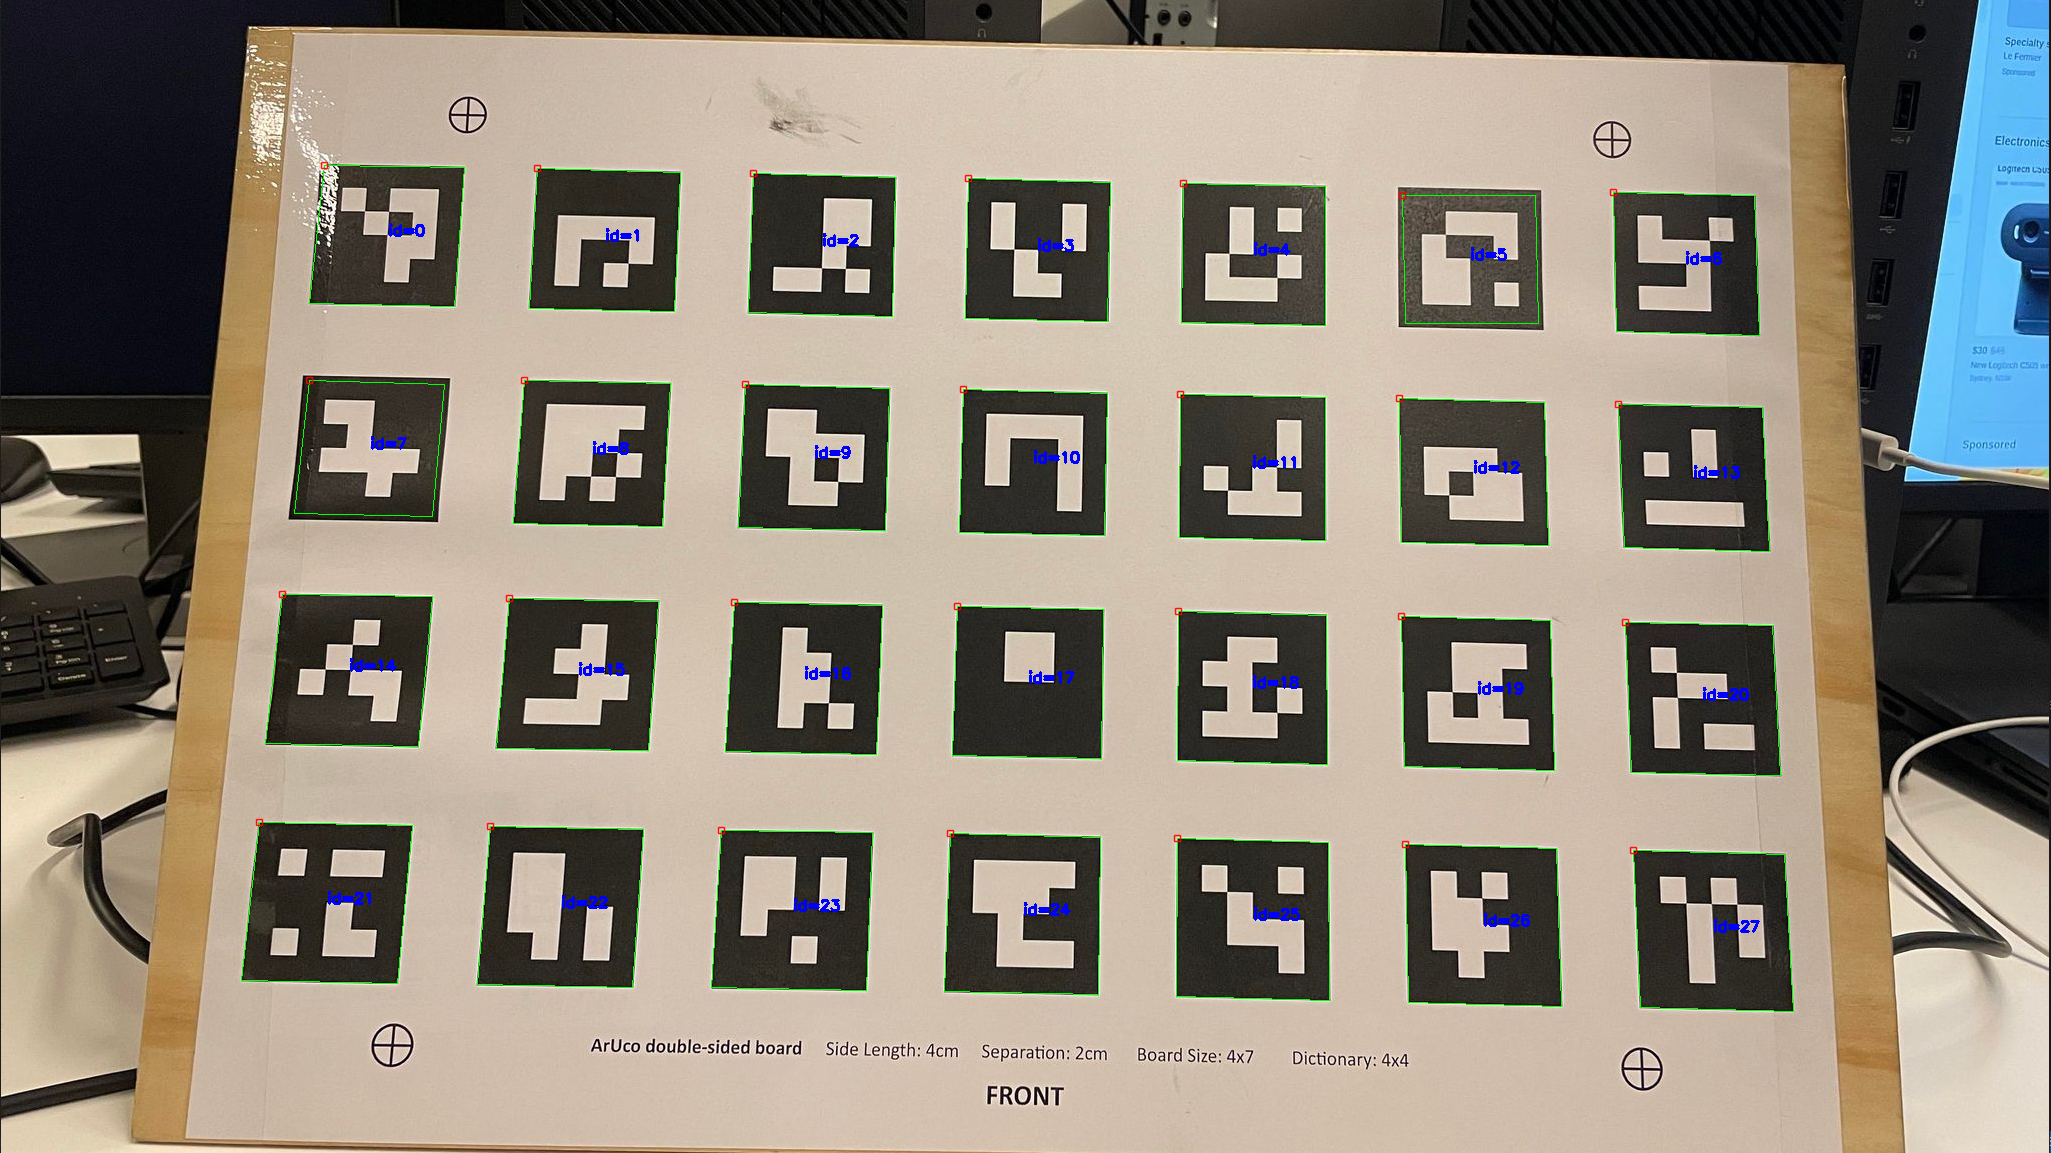
\includegraphics[width=1\textwidth]{Images/ArUco markers detection in image.png}
\caption{ArUco markers detection in image}
\end{figure}

After detecting markers and their IDs on the image, we have to determine their corresponding 3D points respected to ArUco board pose. As mentioned above (chapter 4.2), we already have had a list of markers' corner 3D coordinates (the object points) initialising by MATLAB. Based on the list of markers detected on the image and their IDs, we can define their relative 3D point coordinates in the board's origin frame (see Table \ref{tab:boardconfig}). Finally, after detecting the image points and the object points of ArUco markers, we should combine them with the intrinsic parameters of the respective camera (see Table \ref{tab:intrinsic}). Using the solvePnP() function, we can calculate the 3D rotation and translation vector from the ArUco board pose to the respective camera, and then estimate the relative pose between them. The demonstration of the ArUco board estimation process is shown below.

\begin{figure}[ht]
\centering
\includegraphics[width=0.7\textwidth]{Images/Board detection (front).jpg}
\caption{ArUco board estimation (front side)}
\end{figure}

\begin{figure}[ht]
\centering
\includegraphics[width=0.7\textwidth]{Images/Board detection (back).jpg}
\caption{ArUco board estimation (back side)}
\end{figure}

\clearpage
\section{Pose Graph Optimisation}
After estimating the relative pose between the double-sided ArUco board and each camera in the system, we separated the transformation into translation and rotation. The translation is presented as 3D vectors $[t_{x}, t_{y}, t_{z}]$, and the rotation is demonstrated as the quaternion formula $[q_{x}, q_{y}, q_{z}, q_{w}]$. We captured a total of 1652 images during the calibration process, which means each camera captured 413 photos of the ArUco board.

To implement the pose graph optimisation, we saved the estimated translation vectors and rotation quaternions of the whole calibration process as two CSV files: Nodes.csv and Edges.csv. 

One CSV file contained the nodes of the pose graph, including four nodes of cameras and 413 nodes of image poses. Camera 7 is the origin node, with the default value $[t_{x}, t_{y}, t_{z}] = [0, 0, 0]$ and $[q_{x}, q_{y}, q_{z}, q_{w}] = [0, 0, 0, 1]$. The remaining three camera nodes are the initial guess relative poses, which are measured directly from the multi-camera system. Finally, the image pose nodes are the transformations of the board's pose to the origin node, camera 7, which are estimated in the previous stage.

The other CSV file included the edges of the graph, which are the relative between nodes in the graph. We presented the edges between camera nodes and image pose nodes, which are the extrinsic parameters of each camera estimated from the ArUco board. In case the camera in our system could not detect the board, we used the last known pose of the previous detectable image. The edge values are also saved as 3D vectors $[t_{x}, t_{y}, t_{z}]$, and the rotation is demonstrated as the quaternion formula $[q_{x}, q_{y}, q_{z}, q_{w}]$.

\clearpage
\begin{figure}[ht]
\centering
\includegraphics[width=1\textwidth]{Images/CSV Nodes.png}
\caption{Nodes CSV file}
\end{figure}

In the Nodes.csv file, the rows list the nodes present in the pose graph and the transformation between the first node (node 7) and the corresponding node in this row. The columns describe the transformation components, including 3D translation vectors $[t_{x}, t_{y}, t_{z}]$ and rotation quaternion $[q_{x}, q_{y}, q_{z}, q_{w}]$. 

\clearpage
\begin{figure}[ht]
\centering
\includegraphics[width=0.9\textwidth]{Images/CSV Edges.jpg}
\caption{Edges CSV file}
\end{figure}

In the Edges.csv file, the first two columns represent two nodes of each edge, and the remaining columns are the relative poses between these two nodes.

\clearpage
After completing the two CSV files containing nodes and edges of the pose graph, we started the optimisation process. For testing purposes, we prepared a MATLAB script to run the pose graph optimisation algorithm because MATLAB can display the result as charts and histograms for easy follow-up. The MATLAB script reads the extrinsic parameters data set in the two CSV files, with the support of the Optimisation Toolbox of MATLAB, calculating the most optimal relative pose from more than 400 transformations between each camera and board's poses. The optimisation results are demonstrated in the figures below.

\begin{table}[ht]
    \caption{\label{tab:result}Pose Graph Optimisation result}
    \begin{tabular}{ |c|c|c|c|c|c|c|c| }
     \hline
    Cam & $t_{x}$ & $t_{y}$ & $t_{z}$ & $q_{x}$ & $q_{y}$ & $q_{z}$ & $q_{w}$ \\
     \hline
    7  & 0 & 0 & 0 & 0 & 0 & 0 & 1 \\ 
    8  & -0.3963  & -0.018545 & 0.0095207 & -0.0070655 & -0.0068763 & 0.0057706 & 0.99993 \\
    9  & -0.79415 & -0.025504 & 0.0021866 & -0.0070058 & -0.0088555 & 0.0090403 & 0.9999  \\ 
    10 & -1.0534  & -0.024433 & 0.17173   & -0.023018  & 0.25748    & 0.0039374 & 0.966   \\ 
     \hline
    \end{tabular}
    \begin{tabular}{|l|}
        Sum of residual error before optimising: 335.4759 (mm) \\
        Sum of residual error after optimising: 16.90129 (mm) \\
        \hline
    \end{tabular}
\end{table}

% \clearpage
\begin{figure}[ht]
\centering
\includegraphics[width=1\textwidth]{Images/optimised_pose_cameras.png}
\caption{\centering Poses of the optimised cameras and calibration board. Cam 7, which is coloured in red, is the origin. Every $10^{th}$ pose of the calibration board's origin represented by a 3D axis}
\end{figure}

\begin{figure}[ht]
\centering
\includegraphics[width=1\textwidth]{Images/graph_before_after_optimising.png}
\caption{\centering The pose graph before and after the optimisation is carried out. Blue circles are the nodes, red lines are the edges, and blue lines are loop-closure edges. The four camera nodes have been labelled in blue.}
\end{figure}